\documentclass[11pt]{article}
%%%%%%%%%%%% PREAMBULO %%%%%%%%%%%%%%%%%%
\usepackage[T1]{fontenc}%indica que usamos la ñ
\usepackage[utf8]{inputenc}%indica el tipo de codificación ISO-8859-1 (latin)ó utf8
\usepackage[spanish]{babel}
\title{Informe del práctico 1.}
\usepackage{amsmath}
\usepackage{amssymb,amsfonts,latexsym}
\usepackage{graphicx}
\usepackage{xcolor}
\usepackage{subfigure}%para colocar varias figuras
\usepackage{multicol}
\usepackage{float}%para colocar las tablas como H
\usepackage{array}%dar formato a las tablas
\usepackage{longtable}%dar formato a las tablas
\usepackage{caption}
\usepackage{pdfpages}

%%%%%%%%%%% CONFIGURACION DEL DOCUMENTO %%%%%%%%%%%%%
\usepackage{anysize}%para personalizar el ancho de los margenes
\marginsize{2cm}{2cm}{2cm}{2cm}%izquierda, derecha, arriba, abajo
\usepackage{anyfontsize}

% Para que las referencias sean hipervínculos a las figuras o ecuaciones y
% aparezcan en color
\usepackage[colorlinks=true,plainpages=true,citecolor=blue,linkcolor=blue]{hyperref}
%\usepackage{hyperref} 
% Para agregar encabezado y pie de página
\usepackage{fancyhdr} 
\pagestyle{fancy}
\fancyhf{}
\fancyhead[L]{\footnotesize Maximiliano Bove - Mauricio Vanzulli} %encabezado izquierda
\fancyhead[R]{\footnotesize GPGPU}   % dereecha
\fancyfoot[R]{\footnotesize Práctico 1}  % Pie derecha
\fancyfoot[C]{\thepage}  % centro
\renewcommand{\footrulewidth}{0.4pt}

\usepackage{listings} % Para usar código fuente
\definecolor{dkgreen}{rgb}{0,0.6,0} % Definimos colores para usar en el código
\definecolor{gray}{rgb}{0.5,0.5,0.5} 

\title{Informe de práctico 1}

%%%%%%%%%%% COMIENZO DEL DOCUMENTO %%%%%%%%%%%%
\begin{document}

%%%%%%%%%%%%%%%%%%%%%%%%%%%%%%%%%% PORTADA %%%%%%%%%%%%%%%%%%%%%%%%%%%%%%%%%%%%%%%%%%%%
																					%%%
\begin{center}																		%%%
\newcommand{\HRule}{\rule{\linewidth}{0.5mm}}									%%%\left
 
 %%%

\begin{minipage}{0.48\textwidth} \begin{flushleft}

\includegraphics[scale = 0.5]{logo_FING.jpg}
\end{flushleft}\end{minipage}
\begin{minipage}{0.48\textwidth} \begin{flushright}

\includegraphics[scale = 0.05]{logo_UdelaR.png}
\end{flushright}\end{minipage}
%title
\vspace{4cm}											
\textsc{\huge  \vspace{5px}}\\[1cm]	
%%%
																				%%%
\HRule \\[0.4cm]																	%%%
 \huge \bfseries Informe práctico 1\\[0.4cm]	%%%
 																					%%%
\HRule \\[6.5cm]													\end{center}

\begin{center}	
Maximiliano Bove - Mauricio Vanzulli\\
Curso: Computación de Propósito General en Unidades de Procesamiento Gráfico.\\
{\large \today}																%%%
\end{center}										  						
%%%%%%%%%%%%%%%% FINAL DE LA PORTADA %%%%%%%%%%%%%%%%%%%%%%%%%%%


%%%%%%%%%%%%%%%%%%%%%%
% Direnecia entre cache references y cache misses a que refieren.
%Porque no cambia tantos los tiempos cuando aumentamos el tamaño de la matriz repsecto al valro de n1.
%
%%%%%%%%%%%%%%%%%%%%%%%
\newpage
\subsection*{Plataforma computacional:} 
 Todas las librerías de este trabajo se ejecutaron en un sistema operativo Linux con arquitectura de 64 bits en un procesador i5-8250U a una frecuencia del reloj de 1.6 $GHz$  y una memoria RAM de 8 Gb.

\section*{Ejercicio 1}
Para este apartado se implementaron las funciones de suma estática por fila y columna, etiquetadas con los nombres \emph{ suma\_est\_fil} y \emph{ suma\_est\_col}. Estas computan las operaciones correspondientes a las sumas de todas las filas de la matriz y de todas sus columnas, sin retornar el resultado. Además, se extendieron estas funciones de forma dinámica, permitiendo la variación de recursos utilizados en memoria, haciendo uso de punteros simples. Estas funciones llevan el nombre de \emph{ suma\_din\_fil} y \emph{ suma\_din\_col} para la suma por filas y columnas de la matriz respectivamente. Complementario a esto se implementó la función \emph{suma\_din\_rand} que accede de forma aleatoria a las entradas de la matriz verificando que no se repitan las celdas que se sumaron anteriormente. Esta forma caótica de acceso a memoria no permite al procesador predecir el comportamiento y ejecutar un \emph{cache-prefetch} de optimización anticipada. 

\subsection*{Resultados experimentales}
La cantidad de operaciones y tiempos de ejecución en milisegundos para diferentes tamaños  de una matriz cuadrada $N$ x $N$ considerando sumas estáticas se presenta en la siguiente tabla:
\begin{table}[h!]
    \centering
    \begin{tabular}{||c|c|c|c|c||}
    \hline       
         N        & \emph{ t\_suma\_est\_fil}  & \emph{t\_suma\_est\_col} & \emph{t\_fil\_est} / N$^2$ & \emph{t\_col\_est} / N$^2$ \\\hline\hline
     128 (2$^7$)    &    0.09                    &          0.09    &   549     & 549     \\
     256 (2$^8$)    &    0.38                    &          0.39    &   579     & 595     \\
     512 (2$^9$)    &    1.52                    &          1.53    &   579     & 583      \\
     \hline
    \end{tabular}
    \caption{Tiempos de ejecución en ms y GFlops para las funciones suma dinámicas. }
    \label{Tab:Ej1:sum:est}
\end{table}

Análogamente al considerar sumas dinámicas se obtuvieron los siguientes resultados:

\begin{table}[h!]
    \centering
    \begin{tabular}{||c|c|c|c||}
        \hline
         $N$   & \emph{t\_suma\_din\_fil}  & \emph{t\_suma\_din\_col} & \emph{t\_suma\_din\_rand} \\[0.5ex]  \hline\hline
        128 ($2^{7})$      & 0.09         & 0.09         & 03.78        \\
        256 ($2^{8}$)     & 0.37         & 0.38         & 19.00        \\
        512 ($2^{9}$)     & 1.49         & 1.51         & 87.99        \\
        1024 ($2^{10}$)   & 6.00         & 7.95         & 675.29       \\
        2048 ($2^{11}$)   & 24.11        & 47.02         & 4403.93      \\
        4096 ($2^{12}$)   & 95.88        & 230.86         & 17342.75    \\ 
        \hline
    \end{tabular}
    \caption{Tiempos de ejecución en ms y GFlops para las funciones suma dinámicas. }
    \label{Tab:Ej1:sum:din}
\end{table}

Los tiempos de ejecución de las anteriores rutinas se obtuvieron a partir del \emph{template} disponible en la plataforma EVA. Debido a las incertidumbres inherentes al procesamiento de datos realizado por el procesador que son del orden de milisegundos las medidas de esta magnitud poseen un excesivo error relativo. Para disminuir el error porcentual el código se ejecuto sucesivas veces promediando el tiempo de ejecución. 

\subsection*{Análisis de resultados}

A continuación se describen las diferencias en términos de tiempos de ejecución para las matrices de suma estática, por filas y columnas, presentados en la Tabla \ref{Tab:Ej1:sum:est}. En primer lugar se observa como el tiempo de ejecución aumenta con el tamaño de las matrices, ya que se ve incrementada la cantidad de accesos a memoria. Este costo de sustraer las variables de memoria es de mayor orden que el de realizar una operación algebraica. 

Existe una relación de orden N$^2$ al realizar la suma por filas para los tamaños 256 y 512. No obstante, esta relación no se cumple para un tamaño de 128 utilizando la misma función y tampoco al realizar la suma por columnas. Además, para los mismos valores de $N$ el tiempo de ejecución aumenta levemente al sumar por columnas respecto a sumar por filas. Este comportamiento se observa a partir de tamaños de 256 con diferencias de $1$ ms. Una explicación para este resultado se puede atribuir a la forma consecutiva en que el procesador accede a memoria con los punteros simples. Al realizarse por filas, el acceso a memoria es de manera secuencial mientras que al sumarse por columnas el procesador debe intercalar los indicies de acceso, lo que conlleva a un mayor tiempo de ejecución.

Con relación a la Tabla \ref{Tab:Ej1:sum:din} se aprecia un aumento del tiempo de ejecución al aumentar el tamaño de la matriz para todas las funciones implementadas. Contrastando la suma dinámica por filas y por columnas se evidencia, al igual que para el caso estático, el mayor costo computacional que implica acceder a la matriz por columnas, nuevamente debido al salto de casillas en las lineas del cache. Además, esta diferencia acentúa notoriamente al aumentar el tamaño de la matriz. 

Al cotejar los resultados de \emph{performance} arrojados por la función \emph{t\_suma\_din\_rand} en comparación con el resto de las rutinas, se observa como el costo computacional aumenta de manera considerable. Esto se debe a que el procesador no es capaz de anticipar los índices de acceso a memoria, y por lo tanto ejecutar el \emph{cache prefetch} que le permita optimizar el acceso a partir de un cierto patrón. En este caso se accede de manera aleatoria y no constante, lo que conlleva a un aumento significativo en el tiempo de ejecución. 

\section*{Ejercicio 2}
En este ejercicio se implementaron diferentes funciones para multiplicar dos matrices $(C=A*B)$ cuadradas de tamaño $N$ x $N$. En primer lugar la función \emph{mult\_simple} realiza el producto de matrices usual accediendo a $B$ por columnas y a $A$ por filas. Otra lógica de para consumar el producto de matrices consiste en acceder a ambas por filas e ir realizando sumas parciales; esto se implementó en la función \emph{mult\_fila}. Cuando las matrices son excesivamente grandes podrían exceder el espacio en memoria requerido para su producto, una forma de solucionar el problema es subdividirla por bloques y realizar el producto de estos. Esta técnica, accediendo de la forma tradicional y por filas, se implementó en las funciones \emph{t\_mult\_bl\_simple} y \emph{t\_mult\_bl\_filas} respectivamente. 

\subsection*{Resultados}
En primer lugar se calcularon los tamaños máximos que soporta es capaz de almacenar cada \emph{cache}. Este umbral se encuentra determinado por el tamaño máximo en bytes de cada \emph{cache} indicado con el nombre $T(c_i)$. A su vez, cada matriz posee una entrada tipo \emph{double} que ocupa un tamaño de 8 bytes y se deberán almacenar las tres matrices $ A $, $B$ y $C$. Dadas estas variables el tamaño máximo de matriz $N_{max}$ para el \emph{cache$_i$} esta dado por la siguiente expresión:

\begin{equation}\label{Eq:Nmax}
    N_{max}^i=\sqrt{\frac{\sum _1^i T(c_i)}{3 ~\text{sizeof(double)}}.}    
\end{equation}

\newpage
Aplicando la Ecuación \eqref{Eq:Nmax} para los tres caché se obtuvieron los siguientes resultados:
\begin{table}[h]
    \centering
    \begin{tabular}{||c|c|c|c|c||}
        \hline
           &$L_1$ I  &$L_1$ D & $L_2$ & $L_3$  \\[0.5ex]  \hline\hline
        $Tb_c$      & 32768 & 32768 & 262144 & 6291456   \\
        $N_{max}$    & 36       & 36         & 116 & 525        \\    \hline
    \end{tabular}
    \caption{Tamaño de máximo de matrices para cada \emph{cache}. }
    \label{Tab:Ej2:Nmax}
\end{table}

En función de los valores máximos explicitados en la Tabla \ref{Tab:Ej2:Nmax} se aplicaron estos criterios a los tamaños de matrices descritas en la letra. Los resultados obtenidos se expresan en la tabla a continuación:

\begin{table}[h]
    \centering
    \begin{tabular}{||c|c|c|c||}
        \hline
           N  &3 N$^2$ sizeof(double) & Encaje \emph{cache}   \\[0.5ex]  \hline\hline
        2$^5$  32   & 24576 & Entra en L1   \\ \hline
        2$^6$  64   & 98304 & Entra en L2+L1   \\ \hline
        2$^7$  128   & 393216 & Entra en L3+L2+L1   \\ \hline
        2$^5$  1024   & 25165824 & Excede \emph{cache}   \\ \hline
        2$^5$  1152   & 31850 &Excede \emph{cache}    \\ \hline
        2$^5$  2048   & 100663 & Excede \emph{cache}     \\ \hline
    \end{tabular}
    \caption{Encaje de las matrices en los diferentes \emph{cache}. }
    \label{Tab:Ej2:Nmax}
\end{table}

A continuación se presentan los resultados obtenidos para el análisis de las diferentes funciones de multiplicación implementadas variando el tamaño de las matrices y sus bloques. Para esto se utilizó la herramienta \emph{perf} ejecutando el siguiente comando:

\begin{verbatim}
    sudo perf stat -g -e instructions,cycles,L1-dcache-loads-L1-dcache-loads-misses 
\end{verbatim}


A partir de esta ejecución se relevaron el tiempo de ejecución en milisegundos $t_ms$, la cantidad de operaciones por segundo (GFlops), Las instrucciones por Ciclo del procesador y el porcentaje de \emph{cache-misses}  y \emph{cache-misses-L1}. Los datos obtenidos para todas las funciones se encuentra en la Sección \ref{Anexo}.

Se graficaron los resultados con el objetivo de ilustrar las relaciones entre las diferentes variables de forma pictórica. En primer lugar se estudió el vínculo que existe entre el tamaño de las matrices para la función  \emph{mult\_simple} encontrándose una relación cúbica (verificada con el ratio $\frac{t}{N^3}$) tal y como se muestra en la figura que prosigue:

\begin{figure}[h]
\centering
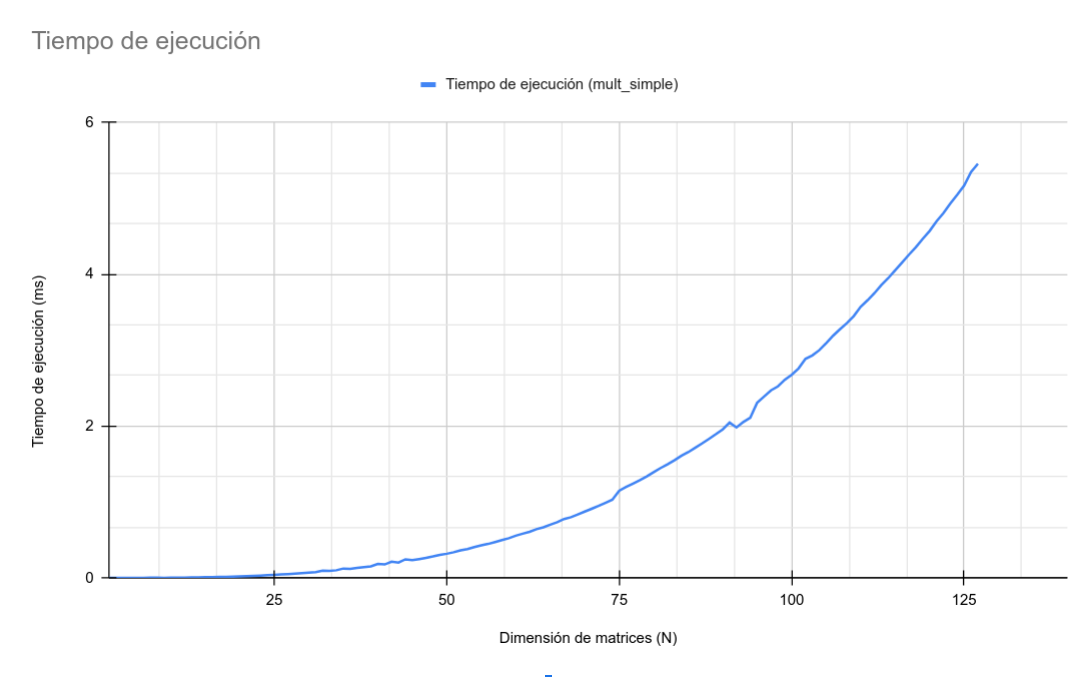
\includegraphics[width=0.5\textwidth]{Ncubo.png}
\caption{Relación tamaño de matriz y tiempo de ejecución.}
\label{Fig:Ej2:Ncubo}
\end{figure}
\newpage
Los resultados de la Figura \ref{Fig:Ej2:Ncubo} se vincularon a la cantidad de operaciones en memoria que requiere la multiplicación tradicional  de matrices es $N^3$. Llevando acabo $N$ veces lectura de datos por columnas de B y $N$ veces columnas de $A$ para luego recorrer $N$ veces las celdas de $C$.

Posteriormente se investigaron las respuestas en términos de desempeño para las funciones de multiplicación variando los  tamaños $N$ de la matriz, hasta 1152. Se analizaron las funciones \emph{mult\_simple} \emph{mult\_fila} según se muestra a continuación:

\begin{figure}[h]
\centering
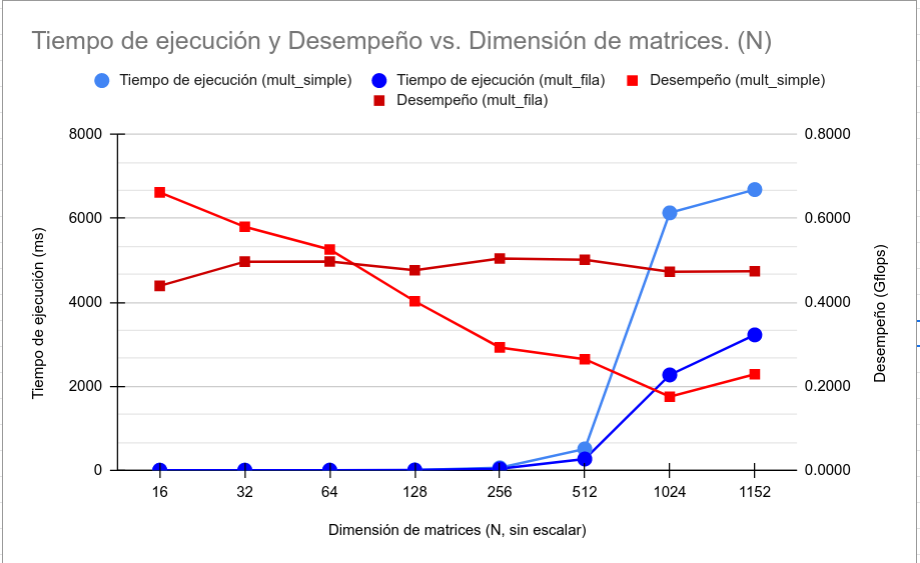
\includegraphics[width=0.6\textwidth]{tiempoYperformanceVSn.png}
\caption{Estudios de desempeño en \emph{mult\_simple} \emph{mult\_fila}.}
\label{Fig:Ej2:DesempenoMult}
\end{figure}

En la Figura \ref{Fig:Ej2:DesempenoMult} se puede confirmar como el tiempo de ejecución se incrementa al aumentar el tamaño de las matrices, de igual modo, la función de multiplicación por filas resuelve el problema en un menor tiempo de ejecución por los argumentos de secuencia de acceso postulados anteriormente. Este resultado también se evidencia al comparar los desempeños en GFlops de la multiplicación simple y por fila. Por otra parte, la multiplicación por filas presenta un desempeño constante mientras que la multiplicación simple decrece con el tamaño de la matriz. Otro comportamiento interesante se observa en el aumento de tiempos de ejecución y la caída de desempeño que se produce al pasar de $N=512$ a $N=1024$. Esto puede deberse al exceso del cache L3 según lo calculado en la Tabla \ref{Tab:Ej2:Nmax}.
\newpage
Una vez analizadas las funciones simples se prosiguió a estudiar como afectan las distribución de bloques a las funciones de multiplicación por bloques en columnas y por filas. Esto se realizó para un tamaño de $N=1152$ variando el tamaño del bloque en el vector $N_b=[16~ 18~ 32~ 64 ~128]$. Para esto se realizó  un profiling de la función \emph{mult\_bl\_simple} registrando la cantidad de GFlops y el tiempo de ejecución según plasmandose en la siguiente figura:

\begin{figure}[hb]
\centering
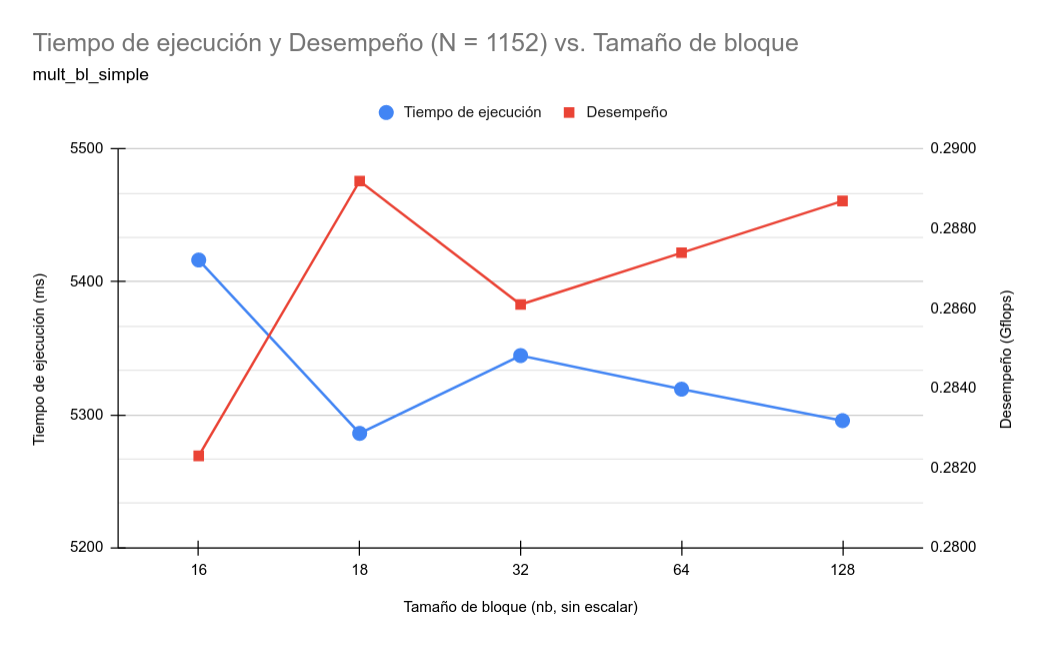
\includegraphics[width=0.5\textwidth]{tiempoYperformance.mult_bl_simple.png}
\caption{Estudios de desempeño en \emph{mult\_simple} \emph{mult\_fila}.}
\label{Fig:Ej2:DesempenoMultSimpleBloque}
\end{figure}

Análogamente se graficaron las mismas variables para la función \emph{mult\_bl\_fil} obteniéndose la siguiente figura:

\begin{figure}[h]
\centering
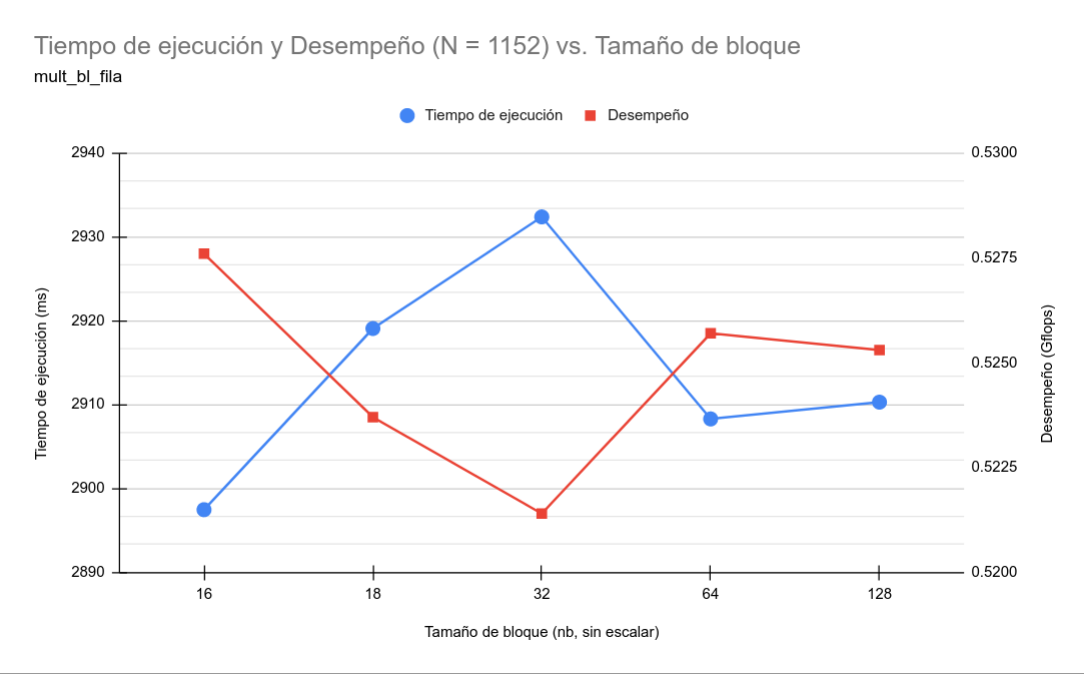
\includegraphics[width=0.6\textwidth]{tiempoYperformance.mult_bl_fila.png}
\caption{Estudios de desempeño en \emph{mult\_simple} \emph{mult\_fila}.}
\label{Fig:Ej2:DesempenoMultFilaBloque}
\end{figure}

En las Figuras \ref{Fig:Ej2:DesempenoMultSimpleBloque} y \ref{Fig:Ej2:DesempenoMultFilaBloque} se observa un leve incremento del desempeño para un tamaño de bloques de 18 en comparación con el resto de los casos. Esto se puede atribuirse al comando \emph{aligned\_alloc} que reserva un determinada cantidad de celdas en memoria para una variable aun no computada. Para el caso del código implementado se guardaron en unidades de 64 bytes.

Al considerar una matriz de $N$ x $N$ se tienen $N^2$ entradas, estas serán divididas en  ($N_b^2$) elementos por bloques resultando un total de subdivisiones igual a $\frac{N_b^2}{N^2}$. A su vez, como cada casilla en memoria posee 64 bytes según lo reservado por el comando  \emph{aligned\_alloc} se utilizarán un total de $\frac{N_b^2}{64N^2}$ casillas. Para el caso de una matriz de 1152 y los diferentes tamaños de bloques se tienen los siguientes valores:
\newpage
\begin{table}[h]
    \centering
    \begin{tabular}{||c|c|c|c|c||}
        \hline
           $N_b$  & N$^2$ & $N_b^2$ &$ N_b^2$/$N^2$ & $N_b^2$/$N^2$64\\[0.5ex]  \hline\hline
          16    & 1327104   & 256  &496.5 & 7.75\\ \hline
          18    & 1327104   & 324  &4096  & 64 \\ \hline
          32    & 1327104   & 1024 & 1296 & 20.25\\ \hline
    \end{tabular}
    \caption{Número de accesos por linea de bloques en memoria.}
    \label{Tab:Ej2:Nmax}
\end{table}

Como el encaje no es entero el procesador dejará espacios vacíos (\emph{padding}) en línea de memoria reservada disminuyendo así el desempeño computacional.



\newpage
\subsection*{Anexo de resultados}\label{Anexo}
\subsubsection*{Función \emph{mult\_simple}}
\begin{figure}[h]
    \centering
    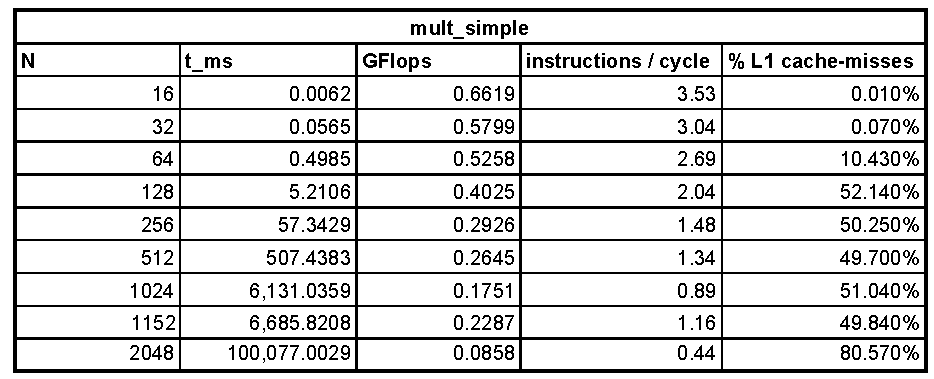
\includegraphics[width=.7\textwidth]{t_mul_simple.pdf}
    \caption{Métricas de la función \emph{mult\_simple}}
    \label{Fig:Ej2:mult_simple}
\end{figure}

\subsubsection*{Función \emph{mult\_fila}}
\begin{figure}[h]
    \centering
    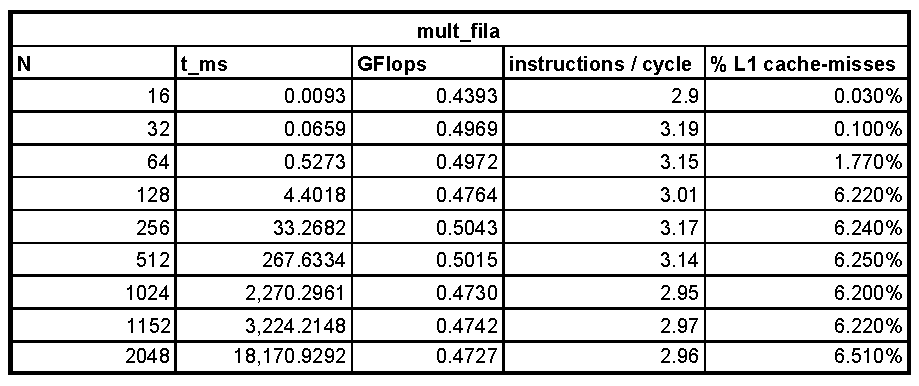
\includegraphics[width=.7\textwidth]{t_mul_fila.pdf}
    \caption{Métricas de la función \emph{mult\_fila}}
    \label{Fig:Ej2:mult_fila}
\end{figure}
\newpage
\subsubsection*{Función \emph{mult\_bl\_simple}}
\begin{figure}[h]
    \centering
    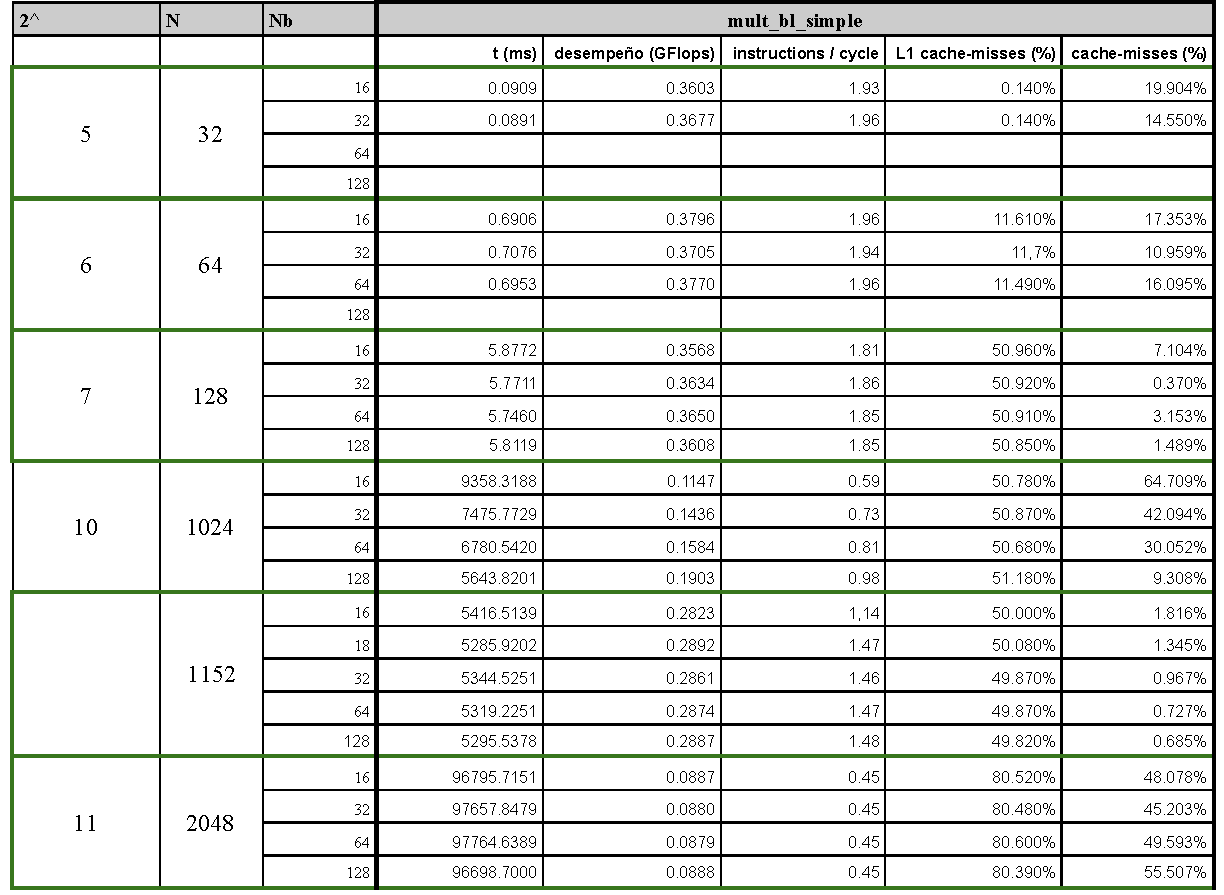
\includegraphics[width=.95\textwidth]{t_mul_bl_simple.pdf}
    \caption{Métricas de la función \emph{mult\_bl\_simple}}
    \label{Fig:Ej2:mult_bl_simple}
\end{figure}
\newpage
\subsubsection*{Función \emph{mult\_bl\_bl}}
\begin{figure}[h]
    \centering
    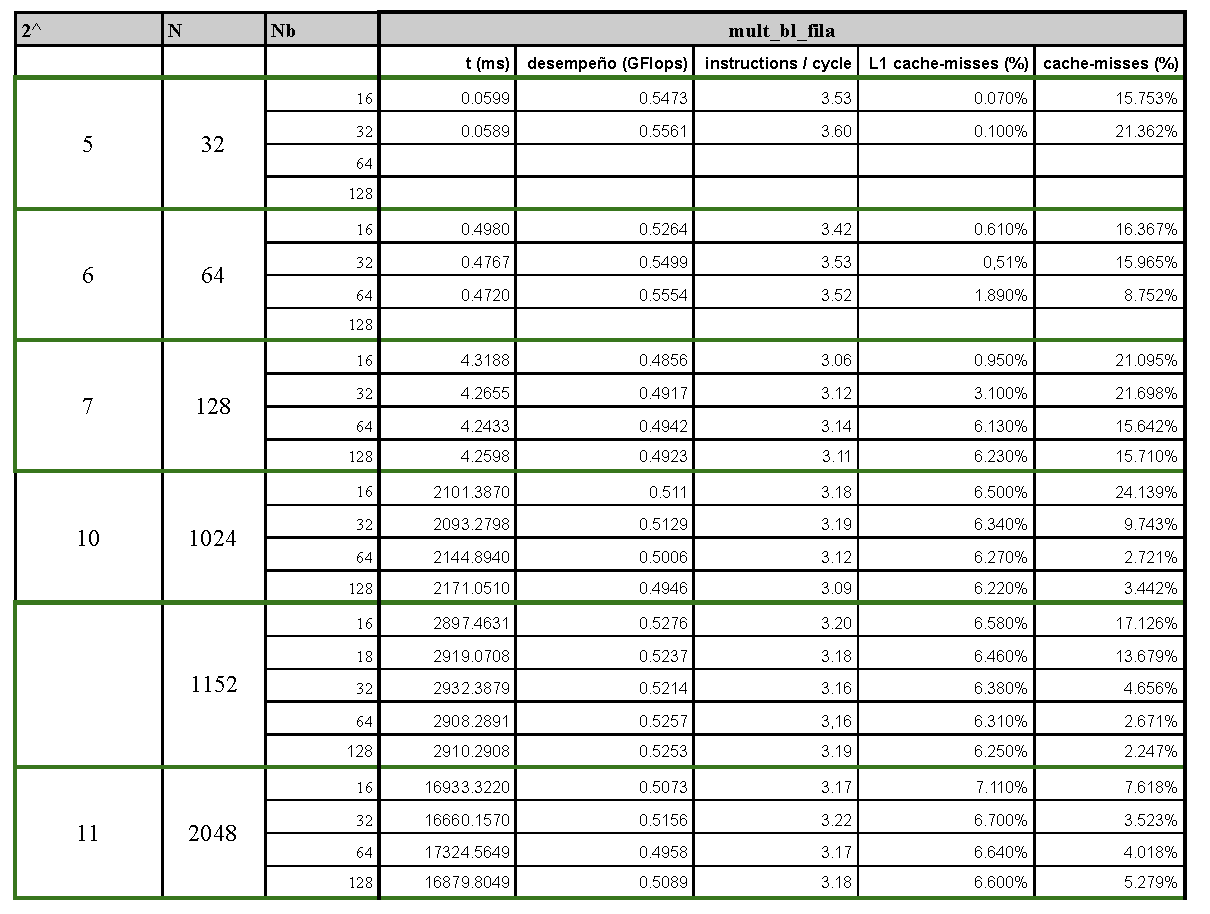
\includegraphics[width=.95\textwidth]{t_mul_bl_fila.pdf}
    \caption{Métricas de la función \emph{mult\_bl\_fila}}
   \label{Fig:Ej2:mult_bl_fila}
\end{figure}

\end{document}

